%%%%%%%%%%%%%%%%%%%%%%%%%%%%%%%%%%

\section{5.5. Comparando médias com ANOVA}

%%%%%%%%%%%%%%%%%%%%%%%%%%%%%%%%%%%

\subsection{Aldrin no rio Wolf}

%%%%%%%%%%%%%%%%%%%%%%%%%%%%%%%%%%%

\begin{frame}
\frametitle{Prática}

\begin{center}
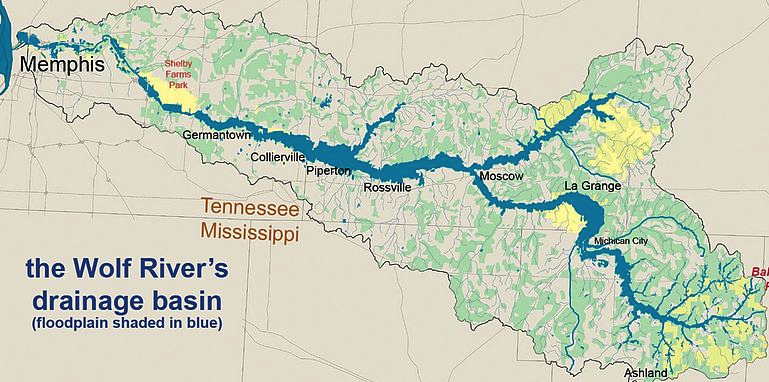
\includegraphics[width=0.7\textwidth]{5-5_anova/wolf.png}
\end{center}

{\small
\begin{itemize}
\justifying
\item O rio Wolf no Tennessee passa por um local abandonado antes utilizado pela indústria de pesticidas para despejar resíduos, incluindo clordano (pesticida), aldrina e dieldrina (ambos inseticidas).

\pause
\justifying
\item Estes compostos orgânicos altamente tóxicos podem causar vários tipos de câncer e problemas congênitos.

\end{itemize}
}
\end{frame}
%%%%%%%%%%%%%%%%%%%%%%%%%%%%%%%%%%%

\begin{frame}
\frametitle{Prática}

{\small
\begin{itemize}
\justifying
\item Os métodos padrão para testar se essas substâncias estão presentes em um rio é coletar amostras a seis décimos de profundidade. 

\pause
\justifying
\item Mas, uma vez que esses compostos são mais densos que a água e suas moléculas tendem a aderir a partículas de sedimento, eles são mais propensos a serem encontrados em concentrações mais altas perto do fundo do que perto da metade da profundidade.

\end{itemize}
}

\end{frame}

%%%%%%%%%%%%%%%%%%%%%%%%%%%%%%%%%%%

\begin{frame}
\frametitle{Dados}
\justifying
Concentração de aldrina (nanogramas por litro) em três níveis de profundidade. \\

\begin{center}
\scalefont{0.7}
\begin{tabular}{r | c | c}
\hline
 	& aldrin 					& depth \\ 
\hline
1 	& \textcolor{darkGray}{3.80} 	& \textcolor{darkGray}{inferior}  \\ 
2 	& \textcolor{darkGray}{4.80} 	& \textcolor{darkGray}{inferior}  \\ 
...	&						& \\
10	& \textcolor{darkGray}{8.80} 	& \textcolor{darkGray}{inferior} \\
11	& \textcolor{blue}{3.20} 		& \textcolor{blue}{meio}  \\
12	& \textcolor{blue}{3.80} 		& \textcolor{blue}{meio} \\
...	&						& \\
20 	& \textcolor{blue}{6.60} 		& \textcolor{blue}{meio} \\
21	& \textcolor{oiB}{3.10} 		& \textcolor{oiB}{superfície} \\
22	& \textcolor{oiB}{3.60} 		& \textcolor{oiB}{superfície} \\
...	&						& \\
30 	& \textcolor{oiB}{5.20} 		& \textcolor{oiB}{superfície} \\  
\hline
\end{tabular}
\end{center}

\end{frame}

%%%%%%%%%%%%%%%%%%%%%%%%%%%%%%%%%%%

\begin{frame}
\frametitle{Análise Exploratória}
\justifying
Concentração de aldrina (nanogramas por litro) em três níveis de profundidade. \\

\begin{center}
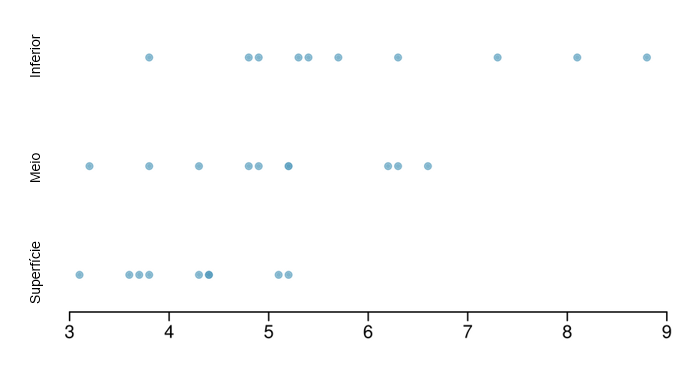
\includegraphics[width=0.65\textwidth]{5-5_anova/dotplot.png}
\end{center}

\begin{center}
\scalefont{0.6}
\begin{tabular}{l | c c c}
		& n	& média	& sd		\\
\hline
inferior	& 10	& 6.04	& 1.58 \\
meio & 10	& 5.05	& 1.10 \\
superficie	& 10	& 4.20	& 0.66 \\
\hline
no geral	& 30	& 5.1	0	& 1.37
\end{tabular}
\end{center}

\end{frame}

%%%%%%%%%%%%%%%%%%%%%%%%%%%%%%%%%%%

\begin{frame}
\frametitle{Questão de pesquisa}
\justifying
\dq{Existe diferença entre as concentrações médias de aldrina entre os três níveis?}

\vspace{0.5cm}

\pause

\begin{itemize}
\justifying
\item Para comparar médias de dois grupos usamos uma estatística Z ou T.

\pause
\justifying
\item Para comparar médias de 3+ grupos, usamos um novo teste chamado \hl{ANOVA} e uma nova estatística chamada \hl{F}.

\end{itemize}

\end{frame}

%%%%%%%%%%%%%%%%%%%%%%%%%%%%%%%%%%%

\begin{frame}
\frametitle{ANOVA}
\justifying
A ANOVA é usada para avaliar se a média da variável é diferente para diferentes níveis de uma variável categórica.

\pause

\begin{itemize}
\justifying
\item[] \mathhl{H_0:} O resultado médio é o mesmo em todas as categorias, 
\[\mu_1 = \mu_2 = \cdots = \mu_k, \]
\justifying
onde $\mu_i$ representa a média do resultado para observações na categoria $i$.
\item[]
\justifying
\item[] \mathhl{H_A:} Pelo menos uma média é diferente das outras.
\end{itemize}

\end{frame}

%%%%%%%%%%%%%%%%%%%%%%%%%%%%%%%%%%%

\begin{frame}
\small
\frametitle{Condições}

\begin{enumerate}
\justifying
\item As observações devem ser independentes dentro e entre os grupos

\begin{itemize}
\justifying
\item Se os dados são provenientes de amostra aleatória simples de menos de 10\% da população, esta condição é satisfeita.
\justifying
\item Verifique com cuidado se os dados podem ser independentes (por exemplo, sem pareamento).
\justifying
\item Sempre importante, mas às vezes difícil de verificar.
\end{itemize}

\pause
\justifying
\item As observações dentro de cada grupo devem ser quase normais.

\begin{itemize}
\justifying
\item Especialmente importante quando os tamanhos das amostras são pequenos.
\end{itemize}
\justifying
\dq{Como podemos verificar a normalidade?}

\pause
\justifying
\item A variabilidade entre os grupos deve ser aproximadamente igual.

\begin{itemize}
\justifying
\item Especialmente importante quando os tamanhos das amostras diferem entre os grupos.
\end{itemize}
\justifying
\dq{Como podemos verificar essa condição?}

\end{enumerate}
\end{frame}


%%%%%%%%%%%%%%%%%%%%%%%%%%%%%%%%%%%

\begin{frame}
\frametitle{$z$/$t$ teste vs. ANOVA - Objetivo}

\twocol{0.5}{0.5}
{\justifying
\[ \hl{$z$/$t$ teste} \]
\justifying
Comparar mpedias de \hl{dois} grupos para ver se elas estão tão distantes que a diferença observada não pode ser atribuída à variabilidade amostral.
\[ H_0: \mu_1 = \mu_2 \]
}
{
\[ \hl{ANOVA} \]
\justifying
Comparar as médias de \hl{dois ou mais} grupos para ver se elas estão tão distantes que as diferenças observadas não podem ser todas atribuídas à variabilidade amostral.
\[ H_0: \mu_1 = \mu_2 = \cdots = \mu_k \]
}

\end{frame}

%%%%%%%%%%%%%%%%%%%%%%%%%%%%%%%%%%%

\begin{frame}
\frametitle{$z$/$t$ teste vs. ANOVA - Método}

\twocol{0.5}{0.5}
{
\[ \hl{$z$/$t$ teste} \]
Calcule uma estatística de teste (uma proporção).
\[ z / t = \frac{(\bar{x}_1 - \bar{x}_2) - (\mu_1 - \mu_2)}{SE(\bar{x}_1 - \bar{x}_2)} \]
}
{
\[ \hl{ANOVA} \]
Calcule uma estatística de teste (uma proporção).
\[ F = \frac{\text{variabilidade entre grupos}}{\text{variabilidade dentro de grupos}} \]
}

\vspace{1cm}

\pause

\begin{itemize}
\justifying
\item Valores grandes das estatísticas de teste levam a valores de p pequenos. 
\justifying
\item Se o valor p for pequeno o suficiente, $H_0$ é rejeitada, concluímos que as médias populacionais não são iguais.

\end{itemize}

\end{frame}

%%%%%%%%%%%%%%%%%%%%%%%%%%%%%%%%%%%

\begin{frame}
\frametitle{$z$/$t$ teste vs. ANOVA}

\begin{itemize}
\justifying
\item Com apenas dois grupos, o teste t e a ANOVA são equivalentes, mas apenas se usarmos uma variância padrão agrupada no denominador da estatística de teste.

\pause
\justifying
\item Com mais de dois grupos, a ANOVA compara as médias amostrais com uma \hl{grande média geral}.

\end{itemize}

\end{frame}

%%%%%%%%%%%%%%%%%%%%%%%%%%%%%%%%%%%

\begin{frame}
\frametitle{Hipóteses}
\justifying
\pq{Quais são as hipóteses corretas para testar a diferença entre as concentrações médias de aldrina entre os três níveis?}

\begin{enumerate}[(a)]
\item $H_0: \mu_B = \mu_M = \mu_S$ \\
$H_A: \mu_B \ne \mu_M \ne \mu_S$ \\
\item $H_0: \mu_B \ne \mu_ M \ne \mu_S$ \\
$H_A: \mu_B = \mu_M = \mu_S$ \\
\solnMult{$H_0: \mu_B = \mu_M = \mu_S$ \\
$H_A:$ Pelo menos uma média é diferente.}
\item $H_0: \mu_B = \mu_M = \mu_S = 0$ \\
$H_A:$ Pelo menos uma média é diferente.
\item $H_0: \mu_B = \mu_M = \mu_S$ \\
$H_A: \mu_B > \mu_M > \mu_S$ \\
\end{enumerate}

\end{frame}

%%%%%%%%%%%%%%%%%%%%%%%%%%%%%%%%%%%

\subsection{ANOVA e o teste F}

%%%%%%%%%%%%%%%%%%%%%%%%%%%%%%%%%%%

\begin{frame}
\frametitle{Estatística de teste}
\justifying
\dq{Parece haver muita variabilidade dentro dos grupos? E que tal entre grupos?}
\justifying
\[ F = \frac{\text{variabilidade entre grupos}}{\text{variabilidade dentro dos grupos}}  \]

\begin{center}
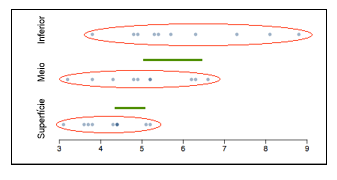
\includegraphics[width=0.75\textwidth]{5-5_anova/dotplot_var.png}
\end{center}

\end{frame}

%%%%%%%%%%%%%%%%%%%%%%%%%%%%%%%%%%%

\begin{frame}
\frametitle{Estatística de teste (cont.)}
\justifying
\[ F = \frac{\text{variabilidade entre grupos}}{\text{variabilidade dentro dos grupos}} = \frac{\hl{MSG}}{\hl{MSE}}  \]

\begin{itemize}
\justifying
\item \hl{MSG} é o quadrado médio entre os grupos
\[ df_G = k - 1 \]
onde $k$ é o número de grupos
\justifying
\item \hl{MSE} é erro quadrático médio - variabilidade dos resíduos
\[ df_E = n - k \]
onde $n$ é o número de observações.

\end{itemize}

\end{frame}
%
%%%%%%%%%%%%%%%%%%%%%%%%%%%%%%%%%%%%

\begin{frame}
\frametitle{$F$ distribuição e valor p}
\justifying
\[ F =  \frac{\text{variabilidade entre grupos}}{\text{variabilidade dentro dos grupos}} \]

\vspace{-1cm}

\begin{center}
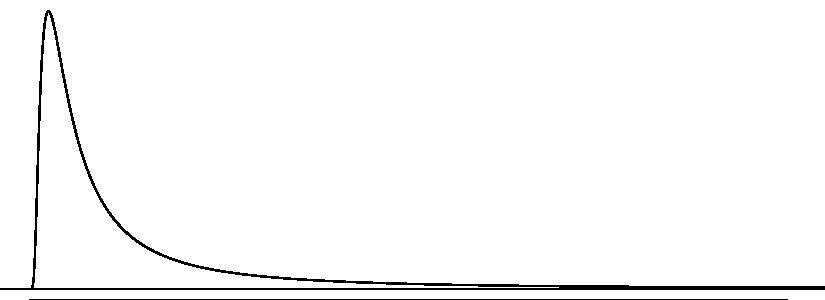
\includegraphics[width=0.75\textwidth]{5-5_anova/fdist.pdf}
\end{center}

\begin{itemize}
\justifying
\item Para podermos rejeitar $ H_0 $, precisamos de um pequeno valor-p, que requer uma estatística F grande.
\justifying
\item Para obter uma estatística F grande, a variabilidade entre as médias da amostra precisa ser maior que a variabilidade dentro das médias amostrais.

\end{itemize}

\end{frame}

%%%%%%%%%%%%%%%%%%%%%%%%%%%%%%%%%%%

\subsection{Saída ANOVA, desconstruída}

%%%%%%%%%%%%%%%%%%%%%%%%%%%%%%%%%%%

\begin{frame}
\frametitle{Graus de liberdade associados à ANOVA}

\vspace{-0.5cm}

{\footnotesize
\begin{center}
\begin{tabular}{ll >{\columncolor[gray]{.6}[.5\tabcolsep]}rrrrr}
\hline
 			& 			& Df 	& Soma Sq	& Média Sq 	& F valor 	& Pr($>$F) \\ 
\hline
(\hl{G}rupo) 	& profundidade 		& 2 	& 16.96 	& 8.48 		& 6.13 	& 0.0063 \\ 
(\hl{E}rro) 	& Resíduos 	& 27 	& 37.33 	& 1.38 		&  		&  \\ 
\hline
	 		& \hl{T}otal	& 29	& 54.29 \\
\end{tabular}
\end{center}
}

\formula{Graus de liberdade associados à ANOVA}
{
\begin{itemize}
\item grupos: $df_G = k - 1$, onde $k$ é o número de grupos
\item total: $df_T = n - 1$, onde $n$ é o tamanho total da amostra
\item erro: $df_E = df_T - df_G$
\end{itemize}
}

\pause

\begin{itemize}

\item $df_G = k - 1 = 3 - 1 = 2$ \\ 

\pause

\item $df_T = n - 1 = 30 - 1 = 29$

\pause

\item $df_E = 29 - 2 = 27$ \\

\end{itemize}

\end{frame}

%%%%%%%%%%%%%%%%%%%%%%%%%%%%%%%%%%%

\begin{frame}
\frametitle{Soma dos quadrados entre os grupos, SSG}

\vspace{-0.25cm}

{\footnotesize
\begin{center}
\begin{tabular}{ll r>{\columncolor[gray]{.6}[.5\tabcolsep]}rrrr}
\hline
 			& 			& Df 	& Soma Sq	& Média Sq 	& F valor 	& Pr($>$F) \\ 
\hline
(\hl{G}rupo) 	& profundidade 		& 2 	& \orange{16.96} 	& 8.48 		& 6.13 	& 0.0063 \\ 
(\hl{E}rro) 	& Resíduos 	& 27 	& 37.33 	& 1.38 		&  		&  \\ 
\hline
	 		& \hl{T}otal	& 29	& 54.29 \\
\end{tabular}
\end{center}
}
\justifying
\formula{Soma dos quadrados entre os grupos, SSG}
{
Mede a variabilidade entre grupos
\vspace{-0.25cm}
\[ SSG = \sum_{i = 1}^{k} n_i (\bar{x}_i - \bar{x})^2 \]
onde $n_i$ é o tamanho de cada grupo, $\bar{x}_i$ é a média para cada grupo, $ \bar {x} $ é a média geral (grande).
}

\end{frame}
%%%%%%%%%%%%%%%%%%%%%%%%%%%%%%%%%%%

\begin{frame}
\frametitle{Soma dos quadrados entre os grupos, SSG}


\vspace{-0.5cm}

\twocol{0.4}{0.5}
{
{\small
\begin{center}
\begin{tabular}{l | c c }
		& n	& média		\\
\hline
inferior	& 10	& 6.04	 \\
meio& 10	& 5.05	 \\
superfície	& 10	& 4.2	 \\
\hline
no geral	& 30	& 5.1	
\end{tabular}
\end{center}
}
}
{
\pause
\begin{eqnarray*}
SSG &=& \pr{ 10 \times (6.04 - 5.1)^2 } \\
\pause
&+& \pr{ 10 \times (5.05 - 5.1)^2 } \\
\pause
&+& \pr{ 10 \times (4.2 - 5.1)^2 } \\
\pause
&=& 16.96 \\
\end{eqnarray*}
}

\end{frame}

%%%%%%%%%%%%%%%%%%%%%%%%%%%%%%%%%%%

\begin{frame}
\frametitle{Soma do total de quadrados SST}

\vspace{-0.25cm}

{\footnotesize
\begin{center}
\begin{tabular}{ll r>{\columncolor[gray]{.6}[.5\tabcolsep]}rrrr}
\hline
 			& 			& Df 	& Soma Sq	& Média Sq 	& F valor 	& Pr($>$F) \\ 
\hline
(\hl{G}rupos) 	& Profundidade 		& 2 	& 16.96	& 8.48 		& 6.13 	& 0.0063 \\ 
(\hl{E}rro) 	& Resíduos 	& 27 	& 37.33 	& 1.38 		&  		&  \\ 
\hline
	 		& \hl{T}otal	& 29	& \orange{54.29} \\
\end{tabular}
\end{center}
}
\justifying
\formula{Soma do total de quadrados SST}
{
Mede a variabilidade entre grupos 
\vspace{-0.25cm}
\[ SST = \sum_{i = 1}^{n} (x_i - \bar{x}) \]
onde $x_i$ representam cada observação no conjunto de dados.
}

\pause

\vspace{-0.75cm}

\begin{eqnarray*}
SST &=& (3.8 - 5.1)^2 + (4.8 - 5.1)^2 + (4.9 - 5.1)^2 + \cdots + (5.2 - 5.1)^2 \\
\pause
&=& (-1.3)^2 + (-0.3)^2 + (-0.2)^2 + \cdots + (0.1)^2 \\
\pause
&=& 1.69 + 0.09 + 0.04 + \cdots + 0.01 \\
\pause
&=& 54.29
\end{eqnarray*}

\end{frame}

%%%%%%%%%%%%%%%%%%%%%%%%%%%%%%%%%%%

\begin{frame}
\frametitle{Soma dos quadrados erro, SSE}

\vspace{-0.25cm}

{\footnotesize
\begin{center}
\begin{tabular}{ll r>{\columncolor[gray]{.6}[.5\tabcolsep]}rrrr}
\hline
 			& 			& Df 	& Soma Sq	& Média Sq 	& F valor 	& Pr($>$F) \\ 
\hline
(\hl{G}rupo) 	& Profundidade 		& 2 	& 16.96	& 8.48 		& 6.13 	& 0.0063 \\ 
(\hl{E}rro) 	& Resíduos 	& 27 	& \orange{37.33} 	& 1.38 		&  		&  \\ 
\hline
	 		& \hl{T}otal	& 29	& 54.29 \\
\end{tabular}
\end{center}
}

\formula{Soma dos quadrados erro, SSE}
{
Mede a variabilidade dentro de grupos:
\[ SSE = SST - SSG \]
}

\pause

\[ SSE =  54.29 - 16.96 =  37.33 \]

\end{frame}

%%%%%%%%%%%%%%%%%%%%%%%%%%%%%%%%%%%

\begin{frame}
\frametitle{Erro quadrático médio}

\vspace{-0.25cm}

{\footnotesize
\begin{center}
\begin{tabular}{ll rr>{\columncolor[gray]{.6}[.5\tabcolsep]}rrr}
\hline
 			& 			& Df 	& Soma Sq	& Média Sq 	& F valor 	& Pr($>$F) \\ 
\hline
(\hl{G}rupo) 	& profundidade 		& 2 	& 16.96	& \orange{8.48} 		& 6.13 	& 0.0063 \\ 
(\hl{E}rro) 	& Resíduos 	& 27 	& 37.33 	& \orange{1.38} 		&  		&  \\ 
\hline
	 		& \hl{T}otal	& 29	& 54.29 \\
\end{tabular}
\end{center}
}
\justifying
\formula{Erro quadrático médio}
{
O erro quadrático médio é calculado como a soma dos quadrados divididos pelos graus de liberdade.
}

\pause

\begin{eqnarray*}
MSG &=& 16.96 / 2 = 8.48 \\
\pause
MSE &=& 37.33 / 27 = 1.38
\end{eqnarray*}

\end{frame}

%%%%%%%%%%%%%%%%%%%%%%%%%%%%%%%%%%%

\begin{frame}
\frametitle{Estatística de teste, valor F}

\vspace{-0.25cm}

{\footnotesize
\begin{center}
\begin{tabular}{ll rrr>{\columncolor[gray]{.6}[.5\tabcolsep]}rr}
\hline
 			& 			& Df 	& Soma Sq	& Média Sq 	& F valor 	& Pr($>$F) \\ 
\hline
(\hl{G}rupo) 	& Profundidade 		& 2 	& 16.96	& 8.48 		& \orange{6.14} 	& 0.0063 \\ 
(\hl{E}rro) 	& Resíduos 	& 27 	& 37.33 	& 1.38 		&  		&  \\ 
\hline
	 		& \hl{T}otal	& 29	& 54.29 \\
\end{tabular}
\end{center}
}
\justifying
\formula{Estatística de teste, valor F}
{
Como discutimos anteriormente, a estatística F é a razão entre o grupo e a variabilidade dentro do grupo.
\[ F = \frac{MSG}{MSE} \]
}

\pause

\[ F = \frac{8.48}{1.38} = 6.14 \]

\end{frame}

%%%%%%%%%%%%%%%%%%%%%%%%%%%%%%%%%%%

\begin{frame}
\frametitle{valor-p}

\vspace{-0.25cm}

{\footnotesize
\begin{center}
\begin{tabular}{ll rrr>{\columncolor[gray]{.6}[.5\tabcolsep]}rr}
\hline
 			& 			& Df 	& Soma Sq	& Média Sq 	& F valor 	& Pr($>$F) \\ 
\hline
(\hl{G}rupo) 	& profundidade 		& 2 	& 16.96	& 8.48 		& \orange{6.14} 	& 0.0063 \\ 
(\hl{E}rro) 	& Resíduos 	& 27 	& 37.33 	& 1.38 		&  		&  \\ 
\hline
	 		& \hl{T}otal	& 29	& 54.29 \\
\end{tabular}
\end{center}
}
\justifying
\formula{valor-p}
{
O valor-p é a probabilidade de pelo menos uma relação tão grande entre a variabilidade "entre grupo" e "dentro do grupo", se de fato os meios de todos os grupos são iguais. É calculado como a área sob a curva F, com graus de liberdade $df_G$ e $df_E$, acima da estatística F observada.
}

\pause

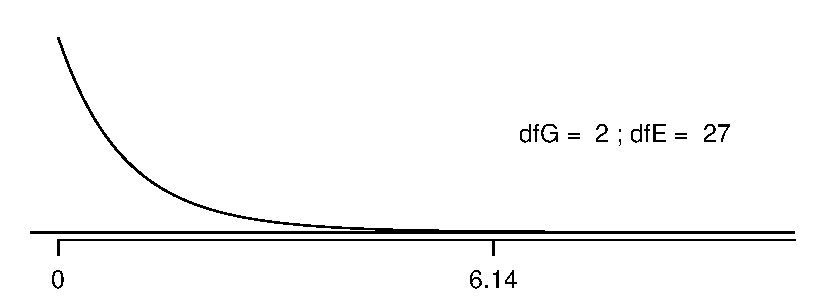
\includegraphics[width=0.5\textwidth]{5-5_anova/f.pdf}

\end{frame}

%%%%%%%%%%%%%%%%%%%%%%%%%%%%%%%%%%%

\begin{frame}
\frametitle{Conclusão - no contexto}
\justifying
\pq{Qual é a conclusão do teste de hipóteses?}

$\:$ \\
\justifying
Os dados fornecem evidências de que a concentração média de aldrina
\begin{enumerate}[(a)]
\justifying
\item  é diferente para todos os grupos.
\justifying
\item na superfície é menor que os outros níveis.
\justifying
\solnMult{é diferente para pelo menos um grupo.}
\justifying
\item é o mesmo para todos os grupos.

\end{enumerate}

\end{frame}

%%%%%%%%%%%%%%%%%%%%%%%%%%%%%%%%%%%

\begin{frame}
\frametitle{Conclusão}

\begin{itemize}
\justifying
\item  Se valor-p for pequeno (menor que $\alpha$), rejeite $H_0$. Os dados fornecem evidências de que pelo menos uma média é diferente (mas não podemos dizer qual).

\pause
\justifying
\item Se o valor p for grande, não rejeite $H_0$. Os dados não fornecem evidências de que pelo menos um par de médias são diferentes umas das outras, as diferenças observadas nas médias amostrais são atribuíveis à variabilidade amostral (ou acaso).

\end{itemize}

\end{frame}

%%%%%%%%%%%%%%%%%%%%%%%%%%%%%%%%%%%

\subsection{Condições de verificação}

%%%%%%%%%%%%%%%%%%%%%%%%%%%%%%%%%%%

\begin{frame}[fragile]
\frametitle{(1) Independência}
\justifying
\dq{Esta condição parece estar satisfeita?}
\justifying
\soln{\only<2>{Neste estudo, não temos razão para acreditar que a concentração de Aldrin não seja independente uma da outra...}}

\end{frame}

%%%%%%%%%%%%%%%%%%%%%%%%%%%%%%%%%%%

\begin{frame}[fragile]
\frametitle{(2) Aproximadamente normal}
\justifying
\dq{Esta condição parece estar satisfeita?}

\begin{center}
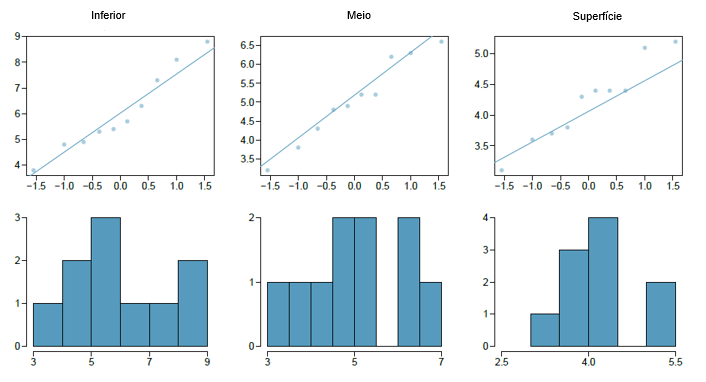
\includegraphics[width=\textwidth]{5-5_anova/normal.png}
\end{center}

\end{frame}

%%%%%%%%%%%%%%%%%%%%%%%%%%%%%%%%%%%

\begin{frame}[fragile]
\frametitle{(3) Variância constante}
\justifying
\dq{Esta condição parece estar satisfeita?}

\begin{center}
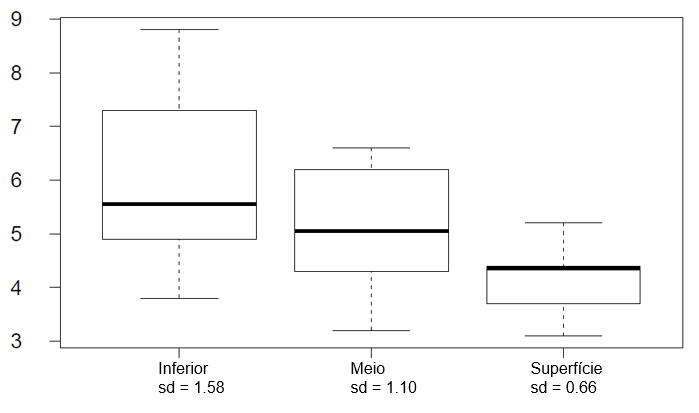
\includegraphics[width=0.7\textwidth]{5-5_anova/homo.png}
\end{center}

\end{frame}

%%%%%%%%%%%%%%%%%%%%%%%%%%%%%%%%%%%

\subsection{Múltiplas comparações \& taxa de erro tipo 1}

%%%%%%%%%%%%%%%%%%%%%%%%%%%%%%%%%%%

\begin{frame}
\frametitle{O que significa diferir?}

\begin{itemize}
\justifying
\item Anteriormente, concluímos que pelo menos um par de médias diferem. A questão natural que se segue é "quais?"

\pause
\justifying
\item Podemos fazer dois testes $ t $ de amostra para diferenças em cada par de grupos possível.

\pause

\end{itemize}
\justifying
\dq{Você consegue ver alguma armadilha com essa abordagem?}

\pause

\begin{itemize}
\justifying
\item Quando executamos muitos testes, a taxa de erro do tipo 1 aumenta.
\justifying
\item Esse problema é resolvido usando um nível de significância modificado.

\end{itemize}

\end{frame}

%%%%%%%%%%%%%%%%%%%%%%%%%%%%%%%%%%%

\begin{frame}
\frametitle{Comparações Múltiplas}

\begin{itemize}
\justifying
\item O cenário de testar muitos pares de grupos é chamado \hl{comparações múltiplas}.

\pause
\justifying
\item A \hl{correção de Bonferroni} sugere que um nível de significância mais \orange{rigoroso} é mais apropriado para estes testes:

\[ \alpha^\star = \alpha / K \]
\justifying
onde $K$ é o número de comparações consideradas.

\pause
\justifying
\item Se existem grupos $k$, então todos os pares possíveis são comparados e $K = \frac{k (k - 1)}{2}$.

\end{itemize}

\end{frame}

%%%%%%%%%%%%%%%%%%%%%%%%%%%%%%%%%%%

\begin{frame}
\frametitle{Determinando o modificado $\alpha$}
\justifying
\pq{No aldrin, a profundidade do conjunto de dados tem 3 níveis: inferior, média e superfície. Se $\alpha = 0.05$, qual deve ser o nível de significância modificado para dois testes $t$ de amostra para determinar quais pares de grupos possuem médias significativamente diferentes?}

\begin{enumerate}[(a)]
\item $\alpha^* = 0.05$
\item $\alpha^* = 0.05 / 2 = 0.025$
\solnMult{$\alpha^* = 0.05 / 3 = 0.0167$}
\item $\alpha^* = 0.05 / 6 = 0.0083$
\end{enumerate}

\end{frame}

%%%%%%%%%%%%%%%%%%%%%%%%%%%%%%%%%%%

\begin{frame}
\frametitle{O que significa diferir?}
\justifying
\pq{Com base nos gráficos abaixo, o que significa que você esperaria ser significativamente diferente?}

\twocol{0.6}{0.4}{
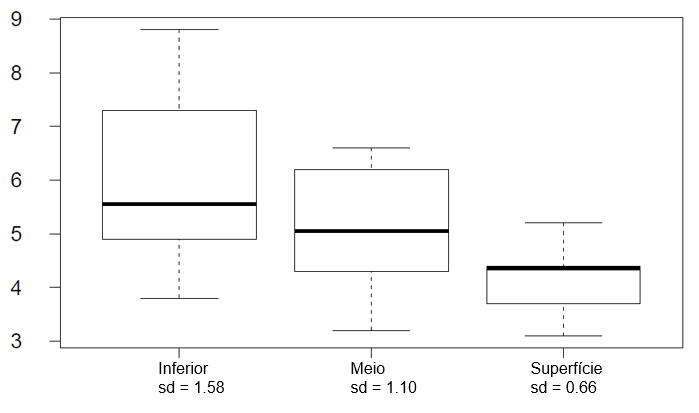
\includegraphics[width=\textwidth]{5-5_anova/homo.png}
}
{
\begin{enumerate}[(a)]
\item inferior \& superfície
\item inferior \& meio
\item meio \& superfície
\item inferior \& meio; meio \& superfície
\item inferior \& meio; inferior \& superfície; meio \& superfície
\end{enumerate}
}

\end{frame}

%%%%%%%%%%%%%%%%%%%%%%%%%%%%%%%%%%

\begin{frame}
\frametitle{O que significa diferir? (cont.)}
\justifying
Se a suposição de variabilidade igual entre os grupos for satisfeita para a ANOVA, podemos usar os dados de todos os grupos para estimar a variabilidade:
 
\begin{itemize}
\justifying
\item Estime qualquer desvio padrão dentro do grupo com $ \sqrt {MSE} $, que é $s_{agrupado}$
\justifying
\item Use os graus de liberdade do erro, $n - k$, para a distribuição $t$.

\end{itemize}
\justifying
\formula{Diferença entre duas médias: após ANOVA}{
\[ SE = \sqrt{  \frac{\sigma_1^2}{n_1} + \frac{\sigma_2^2}{n_2} } \approx \sqrt{ \frac{MSE}{n_1} + \frac{MSE}{n_2} } \]
}

\end{frame}

%%%%%%%%%%%%%%%%%%%%%%%%%%%%%%%%%%

\begin{frame}
\frametitle{Prática}
\justifying
\dq{Existe uma diferença entre a concentração média de aldrina na parte inferior e a meia profundidade?}

\twocol{0.4}{0.7}{
{\scriptsize
\begin{center}
\scalefont{0.8}
\begin{tabular}{l | c c c}
		& n	& média	& sd		\\
\hline
inferior	& 10	& \orange{6.04}	& 1.58 \\
meio& 10	& \orange{5.05}	& 1.10 \\
superfície	& 10	& 4.2 	& 0.66 \\
\hline
no geral	& 30	& 5.1		& 1.37
\end{tabular}
\end{center}
}
}
{
{\scriptsize
\begin{center}
\scalefont{0.8}
\begin{tabular}{l rrrrr}
\hline
 			& Df 	& Soma Sq	& Média Sq 	& F valor 	& Pr($>$F) \\ 
\hline
profundidade 		& 2 	& 16.96 	& 8.48 		& 6.13 	& 0.0063 \\ 
Resíduos 	& \orange{27} 	& 37.33 	& \orange{1.38} 		&  		&  \\ 
\hline
Total			& 29	& 54.29 \\
\end{tabular}
\end{center}
}
}
\scalefont{0.7}
\begin{eqnarray*}
T_{df_E} &=& \frac{(\bar{x}_{inferior} - \bar{x}_{meio})}{\sqrt{ \frac{MSE}{n_{inferior}} + \frac{MSE}{n_{meio}} }} \\ 
\pause
T_{27} &=& \frac{( 6.04 - 5.05 )}{\sqrt{ \frac{1.38}{10} + \frac{1.38}{10} }} = \frac{0.99}{0.53}  =1.87 \\
\pause
0.05 &<& valor-p < 0.10 \qquad \text{{\footnotesize (frente e verso)}} \\
\pause
\alpha^\star &=& 0.05 / 3 = 0.0167
\end{eqnarray*}
\justifying
\pause
{\small Não rejeite $H_0$, os dados não fornecem evidências convincentes de uma diferença entre as concentrações médias de aldrina na profundidade inferior e média.}

\end{frame}

%%%%%%%%%%%%%%%%%%%%%%%%%%%%%%%%%%

\begin{frame}
\frametitle{Prática}
\justifying
\app{Comparações entre pares} {Existe uma diferença entre a concentração média de aldrina no fundo e na superfície?}

\pause

\soln{
\begin{eqnarray*}
T_{df_E} &=& \frac{(\bar{x}_{inferior} - \bar{x}_{superfície})}{\sqrt{ \frac{MSE}{n_{inferior}} + \frac{MSE}{n_{superficie}} }} \\ 
\pause
T_{27} &=& \frac{( 6.04 - 4.02 )}{\sqrt{ \frac{1.38}{10} + \frac{1.38}{10} }} = \frac{2.02}{0.53}  =3.81 \\
\pause
valor-p &<& 0.01 \qquad \text{{\footnotesize (frente e verso)}} \\
\pause
\alpha^\star &=& 0.05 / 3 = 0.0167
\end{eqnarray*}
\pause
\justifying
{\small Rejeite $H_0$, os dados fornecem evidências convincentes de uma diferença entre as concentrações médias de aldrina no fundo e na superfície.}
}

\end{frame}

%%%%%%%%%%%%%%%%%%%%%%%%%%%%%%%%%%

